\documentclass[a4paper]{article}
\usepackage{geometry}
\usepackage{graphicx}
\usepackage{natbib}
\usepackage{amsmath}
\usepackage{amssymb}
\usepackage{amsthm}
\usepackage{paralist}
\usepackage{epstopdf}
\usepackage{tabularx}
\usepackage{longtable}
\usepackage{multirow}
\usepackage{multicol}
\usepackage[hidelinks]{hyperref}
\usepackage{fancyvrb}
\usepackage{algorithm}
\usepackage{algorithmic}
\usepackage{float}
\usepackage{paralist}
\usepackage[svgname]{xcolor}
\usepackage{enumerate}
\usepackage{array}
\usepackage{times}
\usepackage{tikz}
\usepackage{url}
\usepackage{fancyhdr}
\usepackage{comment}
\usepackage{environ}
\usepackage{times}
\usepackage{textcomp}
\usepackage{caption}


\urlstyle{rm}

\setlength\parindent{0pt} % Removes all indentation from paragraphs
\theoremstyle{definition}
\newtheorem{definition}{Definition}[]
\newtheorem{conjecture}{Conjecture}[]
\newtheorem{example}{Example}[]
\newtheorem{theorem}{Theorem}[]
\newtheorem{lemma}{Lemma}
\newtheorem{proposition}{Proposition}
\newtheorem{corollary}{Corollary}

\floatname{algorithm}{Procedure}
\renewcommand{\algorithmicrequire}{\textbf{Input:}}
\renewcommand{\algorithmicensure}{\textbf{Output:}}
\newcommand{\abs}[1]{\lvert#1\rvert}
\newcommand{\norm}[1]{\lVert#1\rVert}
\newcommand{\RR}{\mathbb{R}}
\newcommand{\CC}{\mathbb{C}}
\newcommand{\Nat}{\mathbb{N}}
\newcommand{\br}[1]{\{#1\}}
\DeclareMathOperator*{\argmin}{arg\,min}
\DeclareMathOperator*{\argmax}{arg\,max}
\renewcommand{\qedsymbol}{$\blacksquare$}

\definecolor{dkgreen}{rgb}{0,0.6,0}
\definecolor{gray}{rgb}{0.5,0.5,0.5}
\definecolor{mauve}{rgb}{0.58,0,0.82}

\newcommand{\Var}{\mathrm{Var}}
\newcommand{\Cov}{\mathrm{Cov}}

\newcommand{\vc}[1]{\boldsymbol{#1}}
\newcommand{\xv}{\vc{x}}
\newcommand{\Sigmav}{\vc{\Sigma}}
\newcommand{\alphav}{\vc{\alpha}}
\newcommand{\muv}{\vc{\mu}}

\newcommand{\red}[1]{\textcolor{red}{#1}}

\def\x{\mathbf x}
\def\y{\mathbf y}
\def\w{\mathbf w}
\def\v{\mathbf v}
\def\E{\mathbb E}
\def\V{\mathbb V}

% TO SHOW SOLUTIONS, include following (else comment out):
\newenvironment{soln}{
	\leavevmode\color{blue}\ignorespaces
}{}


\hypersetup{
	%    colorlinks,
	linkcolor={red!50!black},
	citecolor={blue!50!black},
	urlcolor={blue!80!black}
}

\geometry{
	top=1in,            % <-- you want to adjust this
	inner=1in,
	outer=1in,
	bottom=1in,
	headheight=3em,       % <-- and this
	headsep=2em,          % <-- and this
	footskip=3em,
}


\pagestyle{fancyplain}
\lhead{\fancyplain{}{Homework 2}}
\rhead{\fancyplain{}{CS 760 Machine Learning}}
\cfoot{\thepage}

\title{\textsc{Homework 2}} % Title

%%% NOTE:  Replace 'NAME HERE' etc., and delete any "\red{}" wrappers (so it won't show up as red)

\author{
	Daniel Szabo \\
	9074769625\\
} 

\date{}

\begin{document}
	
	\maketitle 
	
	\section{Decision Tree Questions}
	
	\begin{enumerate}
		\item The information gain of any split for a node that has every label the same would be zero. This matches one of the stopping criteria, and therefore the node should be a leaf. In particular the algorithm we saw in class would not even find any candidate splits.
		
		\item If the same features have different label values, the algorithm would simply make a leaf and stop. If we were to force a split, the different labels would still be in the same subset of the training set, and therefore the algorithm would continue indefinitely. This experiment could be done with any number ($ >1 $) of training points, in particular $ 2 $:
		
		\begin{tikzpicture}
			\draw (-1.5,0) -- (1.5,0);
			\draw (0,-1.5) -- (0,1.5);
			\draw[color=red] (.5,.5) circle (.03);
			\draw[color=blue] (.5,.5) circle (.03);
		\end{tikzpicture}
	
		Here the single point in the dataset appears twice, once with label `1' and once with the `0' label, although this is hard to plot.
		
		\item The candidate splits for feature $ 0 $ and their corresponding information gain ratios:\\
		Cut 0.0 has gain ratio 0.10051807676021828\\
		Cut 0.05 has gain ratio 0.10051807676021828
		
		Note that a cut at $ 0.0 $ would be the same as $ 0+\epsilon $ for $ \epsilon>0 $ small, as the algorithm breaks ties downwards. This is why the above gain ratios are the same.\\
		The splits and ratios for feature $ 1 $ are:\\
		Cut -1.5 has gain ratio 0.10051807676021828\\
		Cut -0.5 has gain ratio 0.055953759631263526\\
		Cut 5.5 has gain ratio 0.23609960614360798\\
		Cut 6.5 has gain ratio 0.055953759631263526\\
		Cut 7.5 has gain ratio 0.4301569161309808
		
		\item The (simplified) boolean function this tree represents is $ f(x_1, x_2) = (x_2 > 2.0 \lor x_1> 1.0) $, where a label $ 1 $ corresponds to true. The tree is\\
		1. if $ x_1 \leq 1.0: $\\
		2. \qquad if $ x_2 \leq 2.0: $\\
		3. \qquad \qquad $ y=0 $\\
		4. \qquad else:\\
		5. \qquad\qquad $ y=1 $\\
		6. else:\\ 
		7. \qquad $ y=1 $ 
		
		\item \begin{enumerate}
			\item The tree is very simple:\\
			1. if $ x_2 \leq 0.200777: $\\
			2. \qquad $ y=0 $\\
			3. else:\\
			4. \qquad $ y=1 $
			
			\item There is just a horizontal line at $ x_2=0.200777 $; if the point is above this line, it is classified as 1, if it's below, the label is 0. The space is split perfectly in two by a single separating hyperplane.
			
			\item The decision tree is very large and can't really be viewed here\ldots nonetheless here are the first few lines:\\
			1. If $ x_2 \leq 0.9182275 $:\\
			2. \qquad If $ x_1 \leq 0.53287 $:\\
			3. \qquad \qquad If $ x_2 \leq 0.6911515 $:\\
			4. \qquad \qquad \qquad If $ x_2 \leq 0.5338315 $:\\
			5. \qquad \qquad \qquad \qquad y=0.0\\
			6. \qquad \qquad \qquad Else:\\
			7. \qquad \qquad \qquad \qquad If $ x_2 \leq 0.5362020000000001 $:\\
			8. \qquad \qquad \qquad \qquad \qquad y=1.0\\
			9. \qquad \qquad \qquad \qquad Else:\\
			10.\!\qquad \qquad \qquad \qquad \qquad If $ x_2 \leq 0.5533045000000001 $:\\
			11.\!\qquad \qquad \qquad \qquad \qquad \qquad y=0.0\\
			12.\!\qquad \qquad \qquad \qquad \qquad Else:\\
			13.\!\qquad \qquad \qquad \qquad \qquad \qquad If $ x_2 \leq 0.5550665 $:\\
			14.\!\qquad \qquad \qquad \qquad \qquad \qquad \qquad y=1.0\\
			\vdots
			
			\item It seems the points do not match anything our decision tree can decide. They may be scattered completely randomly, which is why the tree is so large. We cannot be certain without visualization.
			
		\end{enumerate}
			
		\item The plot for \texttt{D1.txt}:
		
		\begin{figure}[h!]
			\centering
			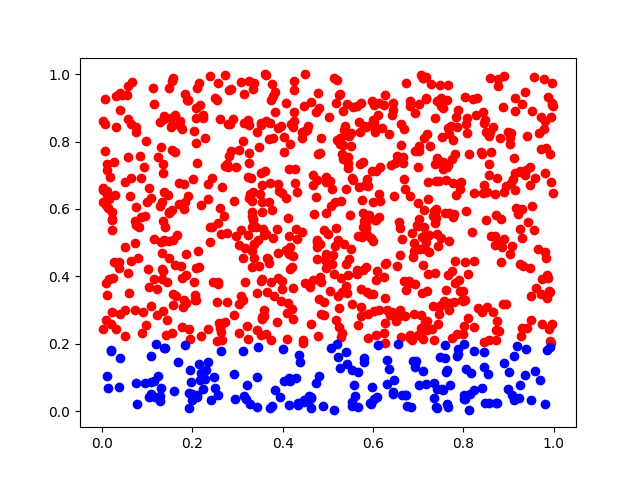
\includegraphics[width=0.4\textwidth]{data/d2plot.png}  
			% reference folder/figure.pdf here and adjust width
			\captionsetup{labelformat=empty}
			\caption{}
			\label{fig:fig1}
		\end{figure}
	And for \texttt{D2.txt}:
	
	\begin{figure}[h!]
		\centering
		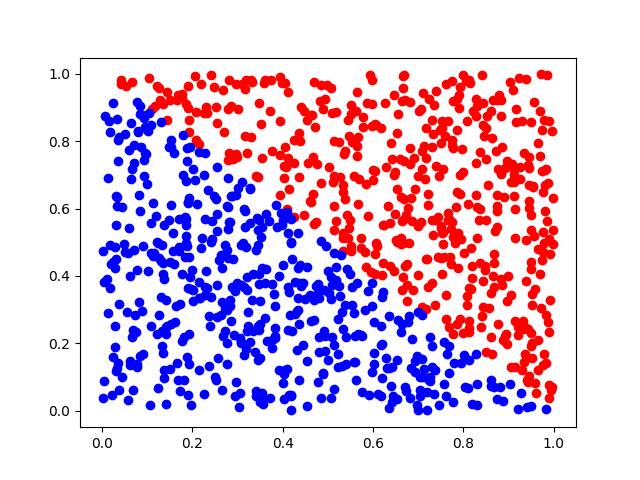
\includegraphics[width=0.4\textwidth]{data/d1plot.png}  
		% reference folder/figure.pdf here and adjust width
		\captionsetup{labelformat=empty}
		\caption{}
		\label{fig:fig2}
	\end{figure}
	This explains why D2 was so incredibly large, as the decision tree can only create horizontal and vertical boundaries, which cannot match the true decision boundary. We have a hypothesis space bias towards these specific vertical or horizontal decision boundaries, rather than arbitrary linear separators.
	
	
	\item The learning curve is:\\
	
	\begin{figure}[h!]
		\centering
		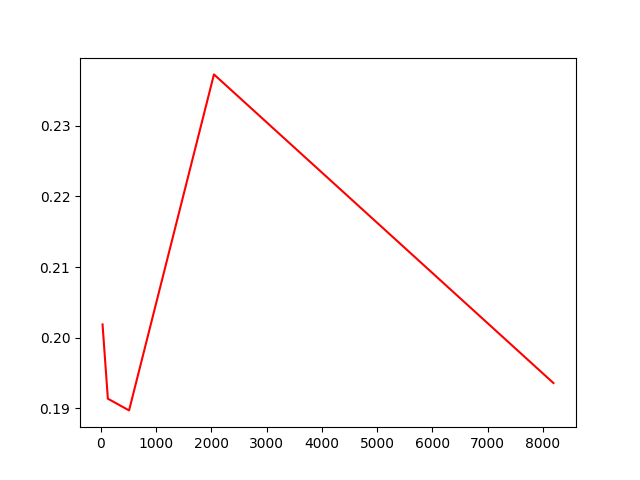
\includegraphics[width=0.4\textwidth]{data/roc.png}
		\captionsetup{labelformat=empty}
		\caption{}
		\label{fig:fig8}
	\end{figure}

\begin{figure}[h!]
	\centering
	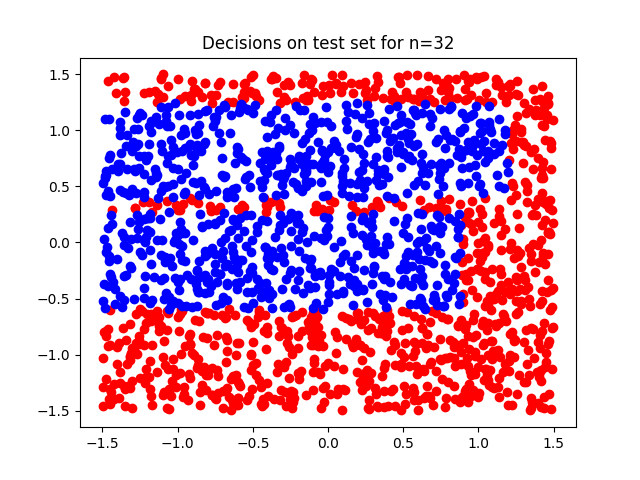
\includegraphics[width=0.4\textwidth]{data/n32.png}
	\captionsetup{labelformat=empty}
	\caption{$ n=32 $, number of nodes=7, $ err_n=0.20188053097345138 $}
	\label{fig:fig3}
\end{figure}

\begin{figure}[h!]
	\centering
	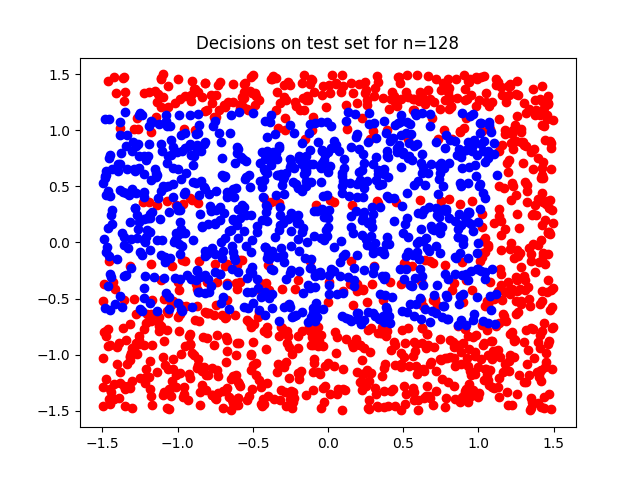
\includegraphics[width=0.4\textwidth]{data/n128.png}
	\captionsetup{labelformat=empty}
	\caption{$ n=128 $, number of nodes=29, $ err_n=0.1913716814159292 $}
	\label{fig:fig4}
\end{figure}

\begin{figure}[h!]
	\centering
	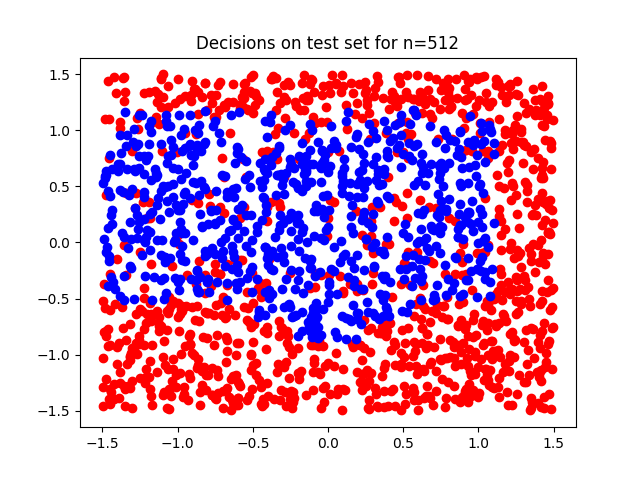
\includegraphics[width=0.4\textwidth]{data/n512.png}
	\caption{$ n=512 $, number of nodes=93, $ err_n=0.18971238938053092 $}
	\label{fig:fig5}
\end{figure}

\begin{figure}[h!]
	\centering
	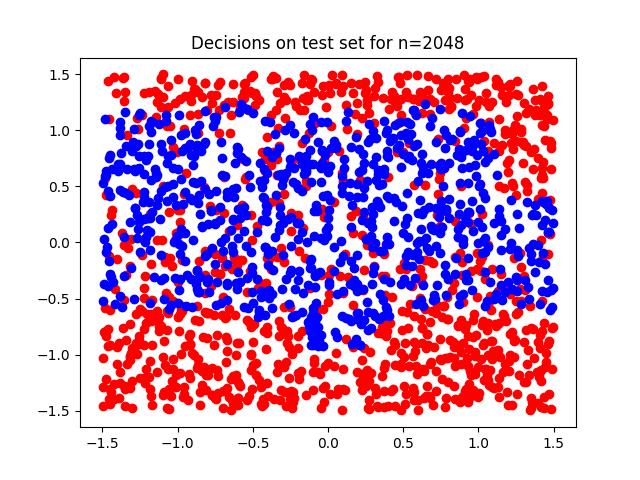
\includegraphics[width=0.4\textwidth]{data/n2048.png}
	\caption{$ n=2048 $, number of nodes=516, $ err_n=0.2372787610619469 $}
	\label{fig:fig6}
\end{figure}

\begin{figure}[h!]
\centering
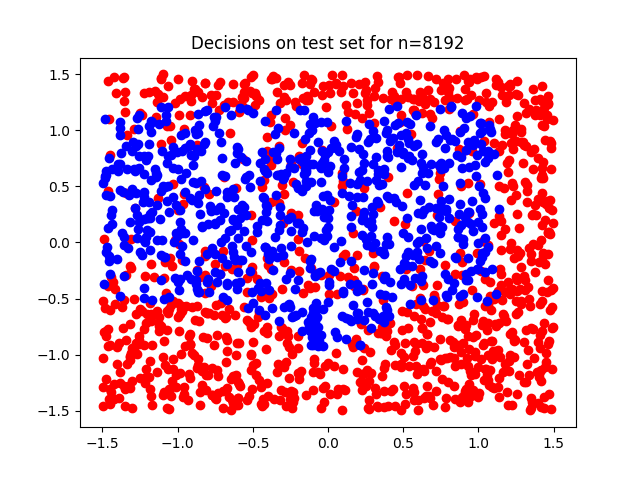
\includegraphics[width=0.4\textwidth]{data/n8192.png}
\caption{$ n=8192 $, number of nodes=1507, $ err_n=0.19358407079646023 $}
\label{fig:fig7}
\end{figure}	
	
	\end{enumerate}

\section{sklearn}


$ n=32 $, number of nodes $ =5 $, $ err_n=0.20630530973451322 $\\
$ n=128 $, number of nodes $ =10 $, $ err_n=0.08683628318584069 $\\
$ n=512 $, number of nodes $ =36 $, $ err_n=0.04646017699115046 $\\
$ n=2048 $, number of nodes $ =62 $, $ err_n=0.02488938053097345 $\\
$ n=8192 $, number of nodes $ =125 $, $ err_n=0.014380530973451378 $\\
The (impressive) learning curve is in Figure \ref{fig:fig9}:

\begin{figure}[h!]
	\centering
	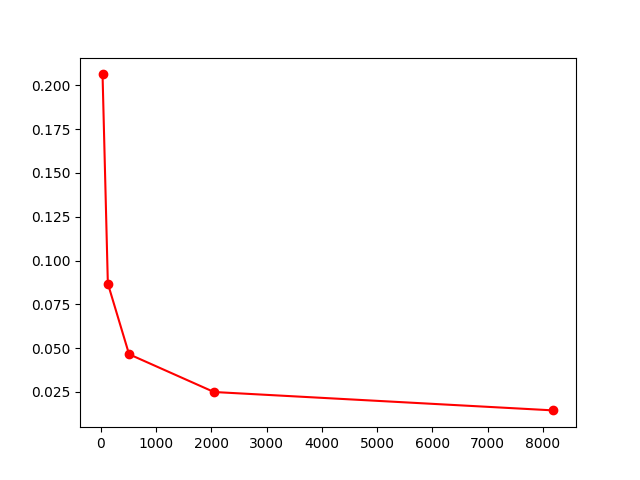
\includegraphics[width=0.4\textwidth]{data/goodroc.png}
	\caption{Learning curve for sklearn's decision tree algorithm}
	\label{fig:fig9}
\end{figure}	

\section{Lagrange Interpolation}

	I sampled 100 points uniformly at random from $ [0,20) $ and computed the training and testing MSEs of Lagrange interpolation to get\\
	Train error (MSE): 0.0\\
	Test error (MSE): 67646250994765.36\\
	Clearly, Lagrange interpolation does not do well on test data, as it has very large coefficients and only performs well at precisely the training points.
	
	Even when we add very small error terms, the error is incredibly huge:\\
	Error for $ \epsilon\sim \mathcal{N}(0,0)^{100}: 0.0 $\\
	Error for $ \epsilon\sim \mathcal{N}(0,10^{-12})^{100}: 735485451224.1586 $\\
	Error for $ \epsilon\sim \mathcal{N}(0,10^{-8})^{100}: 4540211115700.72 $\\
	Error for $ \epsilon\sim \mathcal{N}(0,10^{-6})^{100}: 61576526883137.39 $\\
	Error for $ \epsilon\sim \mathcal{N}(0,0.01)^{100}: 1.2972225357016978e+18 $\\
	Fortunately we see that the error is growing at a polynomial rate, just that the polynomial is very large.
	\bibliographystyle{apalike}
	
	
	%----------------------------------------------------------------------------------------
	
	
\end{document}
